\documentclass[12pt,letterpaper]{article}
\usepackage[latin1]{inputenc}
\usepackage{graphicx}
\usepackage[spanish]{babel}
\usepackage{float}%paquete para flotante, incluir para las imagenes

\begin{document}

{\Huge {\rm { \bf Instituto Politecnico Nacional}}}\\
\begin{center}
{\huge {\rm {\em Escuela Superior de C\'omputo}}} \\
\end{center}
\begin{center}
{\Large {\em Tecnolog\'ias para la Web}}\\
\end{center}
\begin{center}
{\Large Alejandro Hern\'andez Hern\'andez}\\
\end{center}
\begin{center}
{\huge {\bf PR\'ACTICA 7}}
\end{center}

\newpage %nueva pagina
{\Huge {\rm {\bf Introducc\'ion}}}

\vspace{3mm}

{\em Javascript} es un lenguaje de programacion en web, utilizado en el lado del cliente, implementado en navegadores web permitiendo vistas dinamicas y mejras en la interfaz de usuario.
\\Es un lenguaje debilmente tipado y definido como orientado a objetos.
\\El implementar o agregar archivos {\em Javascript}, permite modificar elementos de la pagina html, esto es, agregar, quitar, ocultar, mostrar elementos en una pagina web {\bf sin necesidad de recargar la pagina}, esto define el dinamismo en el lenguaje.

\vspace{2mm}

{\bf Jquery}

\vspace{2mm}

{\em Jquery} es un framework de javascript, cuyo proposito es simplificar el uso y manipulacion del arbol {\bf DOM} de un documento html, manejar eventos y para el uso y desarrollo de animaciones.

\begin{flushleft}

\end{flushleft}

\newpage
{\Huge {\rm {\bf Desarrollo}}}
\begin{flushleft}

Como ya tenemos definido el documento xhtml, esto es, la pagina principal, y el archivo {\em .js} para la dinamica de la pagina, se modificar\'a el archivo, incluyendo el {\em jquery} e implementandolo para conocer su funcionamiento.

\vspace{2mm}

Lo primero, es descargar el archivo de jquery, de la pagina: {\em {\underline {http://jquery.com/download/}}}, personalmente, descargue el {\bf jQuery 3.2.1 slim built}


\begin{figure}[H]%aqui se usa el aquete, notese la H en mayuscula para indicar AQUI quiero la imagen
\begin{minipage}[t]{12cm}
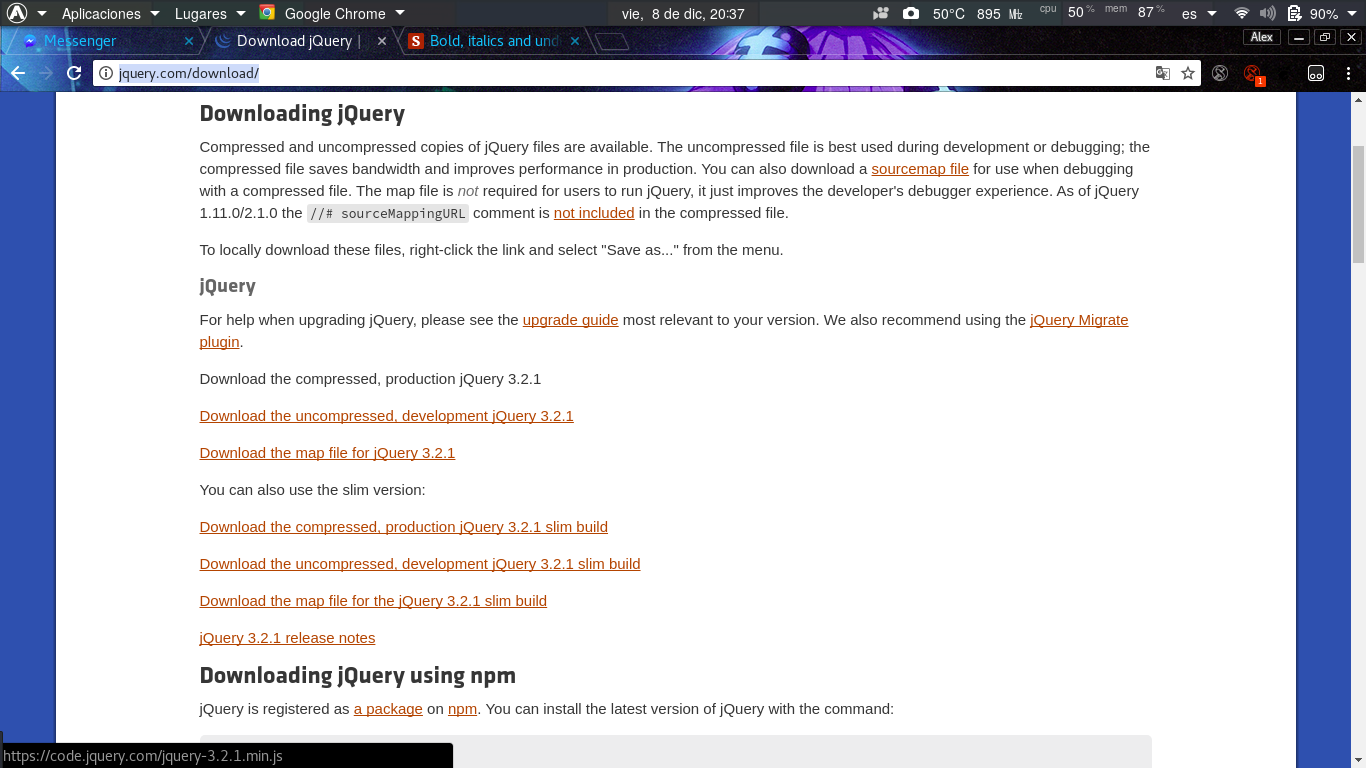
\includegraphics[width=400pt]{./imgs/1.png}
\caption{Descarga jQuery}\label{figura 1}
\end{minipage}
\end{figure}


\vspace{2mm}


una vez descargado, se mueve a la carpeta donde tenemos nuestra calculadora 


\begin{figure}[H]
\begin{minipage}[t]{12cm}
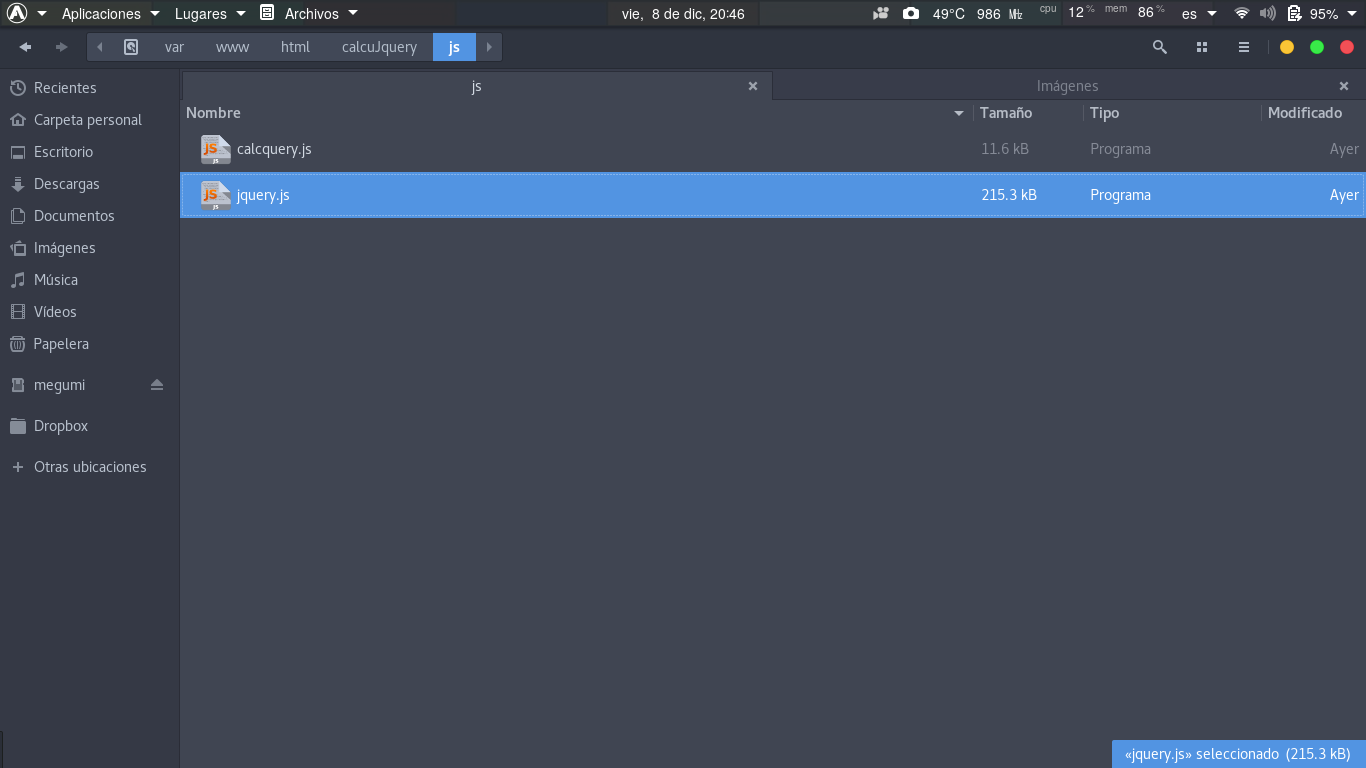
\includegraphics[width=400pt]{./imgs/2.png}
\caption{archivo jquery.js}\label{figura 2}
\end{minipage}
\end{figure}


se incluye en la cabecera como un archivo javascript cualquiera; para fines pr\'acticos, cambi\'e el nombre a {\em jquery.js}


\begin{figure}[H]
\begin{minipage}[t]{12cm}
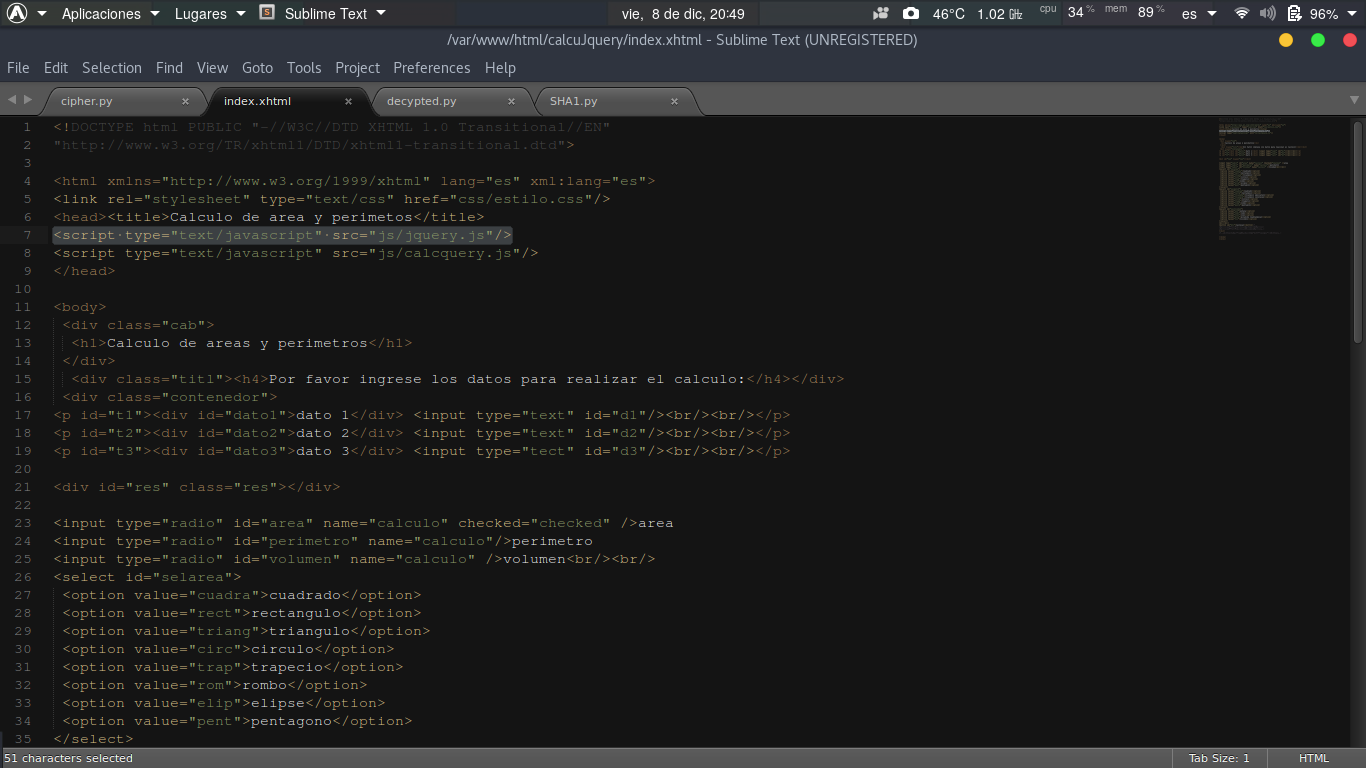
\includegraphics[width=400pt]{./imgs/3.png}
\caption{inclusion jquery.js}\label{figura 3}
\end{minipage}
\end{figure}

\vspace{2mm}
Luego, en el archivo {\em calcquery.js}, agregamos la funcion `principal' que se cargar\'a al mismo tiempo de cargar la pagina


\begin{figure}[H]
\begin{minipage}[t]{12cm}
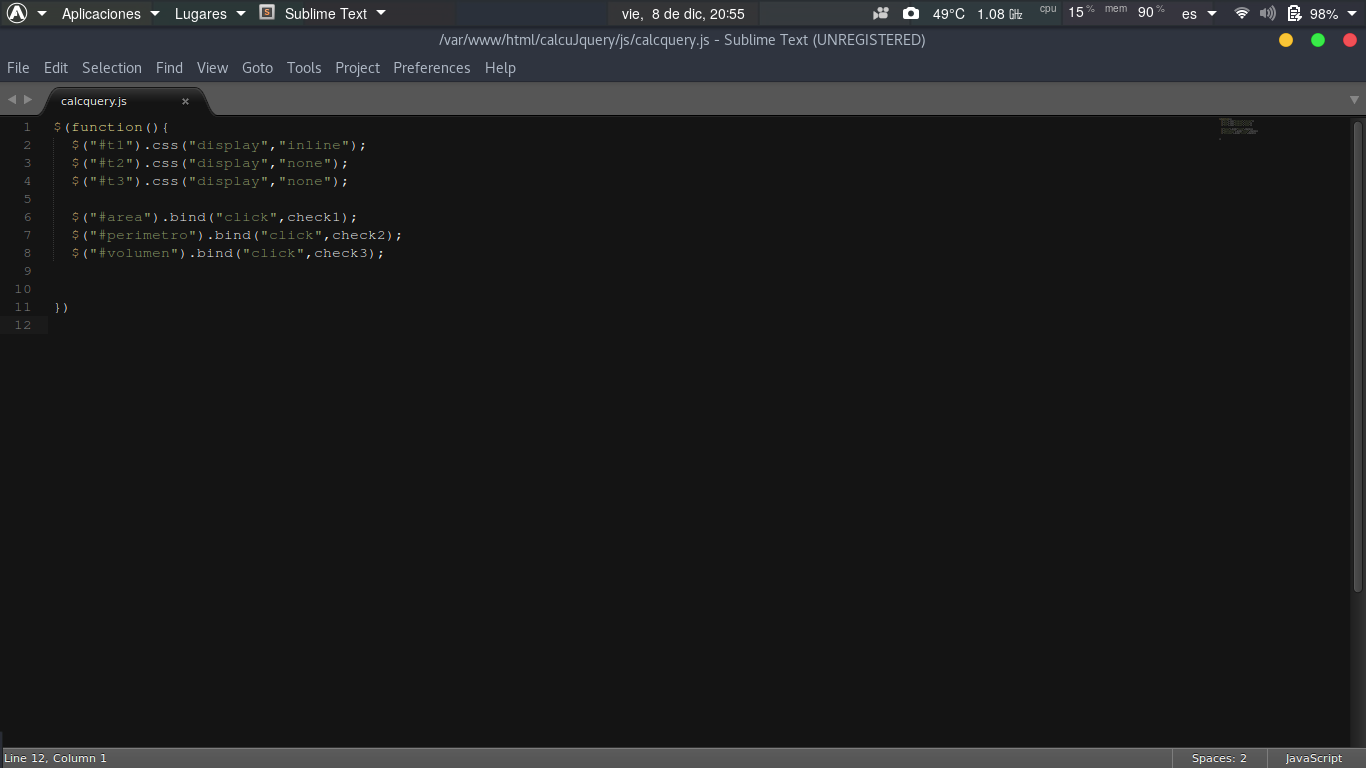
\includegraphics[width=400pt]{./imgs/4.png}
\caption{funcion principal}\label{figura 4}
\end{minipage}
\end{figure}


Luego, sustituimos los llamados o usos de {\em document} en el archivo original de javascript, por {\verb@$(#identificador)@}, y dependiendo de la accion, le seguir\'a, para estilo: {\verb@$(#identificador).css('propiedad','valor');@}; para texto: {\verb@$(#identificador).html("texto a mostrar");@}; para valores en las cajas de entrada: {\verb@$(#identificador).val();@}


\begin{figure}[H]
\begin{minipage}[t]{12cm}
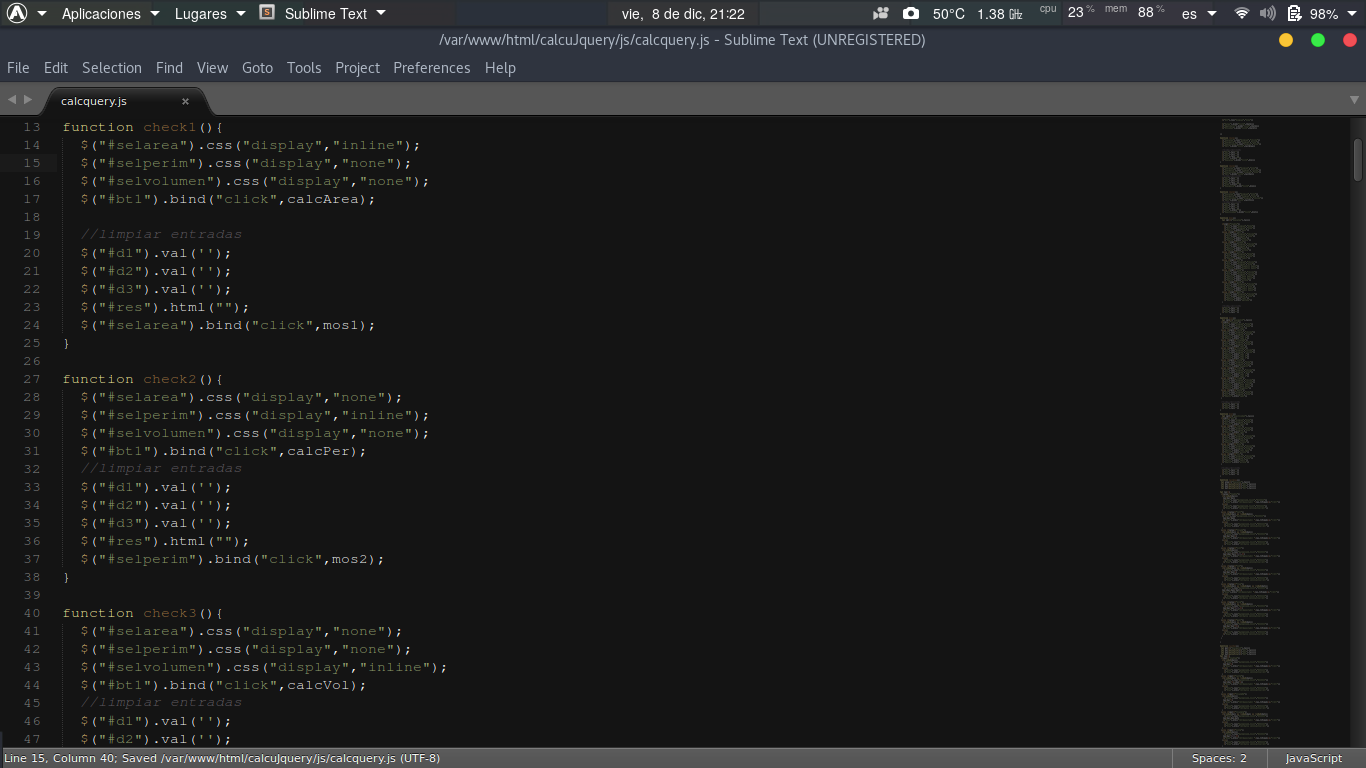
\includegraphics[width=400pt]{./imgs/5.png}
\caption{modificaci\'on}\label{figura 5}
\end{minipage}
\end{figure}

y al comprobar el funcionamiento de la pagina, era exactamente el mismo que con el anterior javascript.

\newpage

{\Huge {\rm {\bf Conclusi\'on}}}

\vspace{2mm}

El uso de jquery, personalmente, me facilit\'o el entendimiento de mi anterior c\'odigo, asi como reducci\'on en el tama\~no de las lineas, es decir, el codigo qued\'o mejor, y se `optimiz\'o' el uso de variables en jquery que en javascript, ademas de que no me bombardee de tando document.getElementById para cambiar estilos de las etiquetas y elementos en el html.\\
En resumen, jquery me permiti\'o manupular el arbol DOM mejor que javascript solo, mandando a llamar solamente el elemento a modificar con el nombre de su identificador.
\end{flushleft}

\end{document}
